% Options for packages loaded elsewhere
\PassOptionsToPackage{unicode}{hyperref}
\PassOptionsToPackage{hyphens}{url}
%
\documentclass[
]{article}
\usepackage{amsmath,amssymb}
\usepackage{iftex}
\ifPDFTeX
  \usepackage[T1]{fontenc}
  \usepackage[utf8]{inputenc}
  \usepackage{textcomp} % provide euro and other symbols
\else % if luatex or xetex
  \usepackage{unicode-math} % this also loads fontspec
  \defaultfontfeatures{Scale=MatchLowercase}
  \defaultfontfeatures[\rmfamily]{Ligatures=TeX,Scale=1}
\fi
\usepackage{lmodern}
\ifPDFTeX\else
  % xetex/luatex font selection
\fi
% Use upquote if available, for straight quotes in verbatim environments
\IfFileExists{upquote.sty}{\usepackage{upquote}}{}
\IfFileExists{microtype.sty}{% use microtype if available
  \usepackage[]{microtype}
  \UseMicrotypeSet[protrusion]{basicmath} % disable protrusion for tt fonts
}{}
\makeatletter
\@ifundefined{KOMAClassName}{% if non-KOMA class
  \IfFileExists{parskip.sty}{%
    \usepackage{parskip}
  }{% else
    \setlength{\parindent}{0pt}
    \setlength{\parskip}{6pt plus 2pt minus 1pt}}
}{% if KOMA class
  \KOMAoptions{parskip=half}}
\makeatother
\usepackage{xcolor}
\usepackage[margin=1in]{geometry}
\usepackage{color}
\usepackage{fancyvrb}
\newcommand{\VerbBar}{|}
\newcommand{\VERB}{\Verb[commandchars=\\\{\}]}
\DefineVerbatimEnvironment{Highlighting}{Verbatim}{commandchars=\\\{\}}
% Add ',fontsize=\small' for more characters per line
\usepackage{framed}
\definecolor{shadecolor}{RGB}{248,248,248}
\newenvironment{Shaded}{\begin{snugshade}}{\end{snugshade}}
\newcommand{\AlertTok}[1]{\textcolor[rgb]{0.94,0.16,0.16}{#1}}
\newcommand{\AnnotationTok}[1]{\textcolor[rgb]{0.56,0.35,0.01}{\textbf{\textit{#1}}}}
\newcommand{\AttributeTok}[1]{\textcolor[rgb]{0.13,0.29,0.53}{#1}}
\newcommand{\BaseNTok}[1]{\textcolor[rgb]{0.00,0.00,0.81}{#1}}
\newcommand{\BuiltInTok}[1]{#1}
\newcommand{\CharTok}[1]{\textcolor[rgb]{0.31,0.60,0.02}{#1}}
\newcommand{\CommentTok}[1]{\textcolor[rgb]{0.56,0.35,0.01}{\textit{#1}}}
\newcommand{\CommentVarTok}[1]{\textcolor[rgb]{0.56,0.35,0.01}{\textbf{\textit{#1}}}}
\newcommand{\ConstantTok}[1]{\textcolor[rgb]{0.56,0.35,0.01}{#1}}
\newcommand{\ControlFlowTok}[1]{\textcolor[rgb]{0.13,0.29,0.53}{\textbf{#1}}}
\newcommand{\DataTypeTok}[1]{\textcolor[rgb]{0.13,0.29,0.53}{#1}}
\newcommand{\DecValTok}[1]{\textcolor[rgb]{0.00,0.00,0.81}{#1}}
\newcommand{\DocumentationTok}[1]{\textcolor[rgb]{0.56,0.35,0.01}{\textbf{\textit{#1}}}}
\newcommand{\ErrorTok}[1]{\textcolor[rgb]{0.64,0.00,0.00}{\textbf{#1}}}
\newcommand{\ExtensionTok}[1]{#1}
\newcommand{\FloatTok}[1]{\textcolor[rgb]{0.00,0.00,0.81}{#1}}
\newcommand{\FunctionTok}[1]{\textcolor[rgb]{0.13,0.29,0.53}{\textbf{#1}}}
\newcommand{\ImportTok}[1]{#1}
\newcommand{\InformationTok}[1]{\textcolor[rgb]{0.56,0.35,0.01}{\textbf{\textit{#1}}}}
\newcommand{\KeywordTok}[1]{\textcolor[rgb]{0.13,0.29,0.53}{\textbf{#1}}}
\newcommand{\NormalTok}[1]{#1}
\newcommand{\OperatorTok}[1]{\textcolor[rgb]{0.81,0.36,0.00}{\textbf{#1}}}
\newcommand{\OtherTok}[1]{\textcolor[rgb]{0.56,0.35,0.01}{#1}}
\newcommand{\PreprocessorTok}[1]{\textcolor[rgb]{0.56,0.35,0.01}{\textit{#1}}}
\newcommand{\RegionMarkerTok}[1]{#1}
\newcommand{\SpecialCharTok}[1]{\textcolor[rgb]{0.81,0.36,0.00}{\textbf{#1}}}
\newcommand{\SpecialStringTok}[1]{\textcolor[rgb]{0.31,0.60,0.02}{#1}}
\newcommand{\StringTok}[1]{\textcolor[rgb]{0.31,0.60,0.02}{#1}}
\newcommand{\VariableTok}[1]{\textcolor[rgb]{0.00,0.00,0.00}{#1}}
\newcommand{\VerbatimStringTok}[1]{\textcolor[rgb]{0.31,0.60,0.02}{#1}}
\newcommand{\WarningTok}[1]{\textcolor[rgb]{0.56,0.35,0.01}{\textbf{\textit{#1}}}}
\usepackage{graphicx}
\makeatletter
\def\maxwidth{\ifdim\Gin@nat@width>\linewidth\linewidth\else\Gin@nat@width\fi}
\def\maxheight{\ifdim\Gin@nat@height>\textheight\textheight\else\Gin@nat@height\fi}
\makeatother
% Scale images if necessary, so that they will not overflow the page
% margins by default, and it is still possible to overwrite the defaults
% using explicit options in \includegraphics[width, height, ...]{}
\setkeys{Gin}{width=\maxwidth,height=\maxheight,keepaspectratio}
% Set default figure placement to htbp
\makeatletter
\def\fps@figure{htbp}
\makeatother
\setlength{\emergencystretch}{3em} % prevent overfull lines
\providecommand{\tightlist}{%
  \setlength{\itemsep}{0pt}\setlength{\parskip}{0pt}}
\setcounter{secnumdepth}{-\maxdimen} % remove section numbering
\ifLuaTeX
  \usepackage{selnolig}  % disable illegal ligatures
\fi
\IfFileExists{bookmark.sty}{\usepackage{bookmark}}{\usepackage{hyperref}}
\IfFileExists{xurl.sty}{\usepackage{xurl}}{} % add URL line breaks if available
\urlstyle{same}
\hypersetup{
  pdftitle={SoilMercury data example},
  pdfauthor={ruoyong},
  hidelinks,
  pdfcreator={LaTeX via pandoc}}

\title{SoilMercury data example}
\author{ruoyong}
\date{2023-04-22}

\begin{document}
\maketitle

\begin{Shaded}
\begin{Highlighting}[]
\FunctionTok{library}\NormalTok{(}\StringTok{\textquotesingle{}terra\textquotesingle{}}\NormalTok{)}
\end{Highlighting}
\end{Shaded}

\begin{verbatim}
## terra 1.7.65
\end{verbatim}

\begin{Shaded}
\begin{Highlighting}[]
\FunctionTok{load}\NormalTok{(}\StringTok{"hgmTerra.RData"}\NormalTok{)}
\NormalTok{hgm }\OtherTok{=} \FunctionTok{unwrap}\NormalTok{(hgmWrap)}
\NormalTok{myBgMap }\OtherTok{=}\NormalTok{ mapmisc}\SpecialCharTok{::}\FunctionTok{openmap}\NormalTok{(hgm, }\AttributeTok{zoom=}\DecValTok{2}\NormalTok{)}


\FunctionTok{load}\NormalTok{(}\StringTok{"covListWrap.RData"}\NormalTok{)}
\NormalTok{covList }\OtherTok{=} \FunctionTok{lapply}\NormalTok{(covListWrap, unwrap)}
\FunctionTok{names}\NormalTok{(covList) }\OtherTok{=} \FunctionTok{gsub}\NormalTok{(}\StringTok{"Wrap"}\NormalTok{, }\StringTok{""}\NormalTok{, }\FunctionTok{names}\NormalTok{(covList))}


\NormalTok{world1 }\OtherTok{=} \FunctionTok{crop}\NormalTok{(}\FunctionTok{vect}\NormalTok{(rnaturalearth}\SpecialCharTok{::}\FunctionTok{ne\_countries}\NormalTok{(}\AttributeTok{scale=}\StringTok{\textquotesingle{}medium\textquotesingle{}}\NormalTok{, }\AttributeTok{returnclass=}\StringTok{\textquotesingle{}sf\textquotesingle{}}\NormalTok{)),}
              \FunctionTok{ext}\NormalTok{(}\SpecialCharTok{{-}}\DecValTok{20}\NormalTok{, }\DecValTok{100}\NormalTok{, }\DecValTok{0}\NormalTok{, }\DecValTok{85}\NormalTok{))}
\NormalTok{worldMap }\OtherTok{=} \FunctionTok{project}\NormalTok{(world1, mapmisc}\SpecialCharTok{::}\NormalTok{crsLL)}
\end{Highlighting}
\end{Shaded}

\begin{figure}
\subfloat[hg\label{fig:firstPlot-1}]{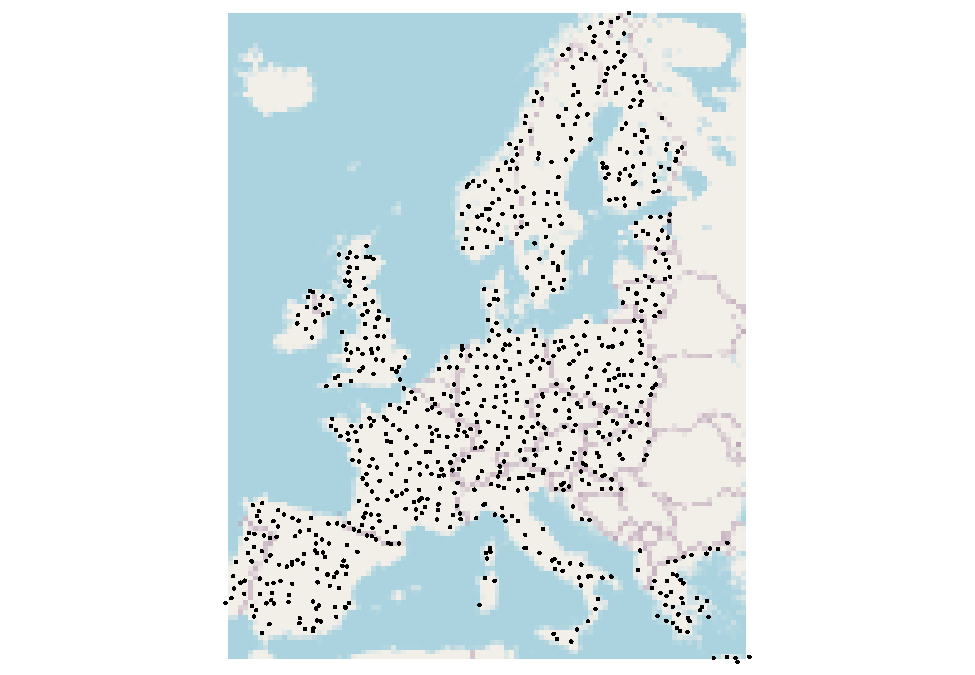
\includegraphics{newsoilsupp_files/figure-latex/firstPlot-1} }\subfloat[elevation\label{fig:firstPlot-2}]{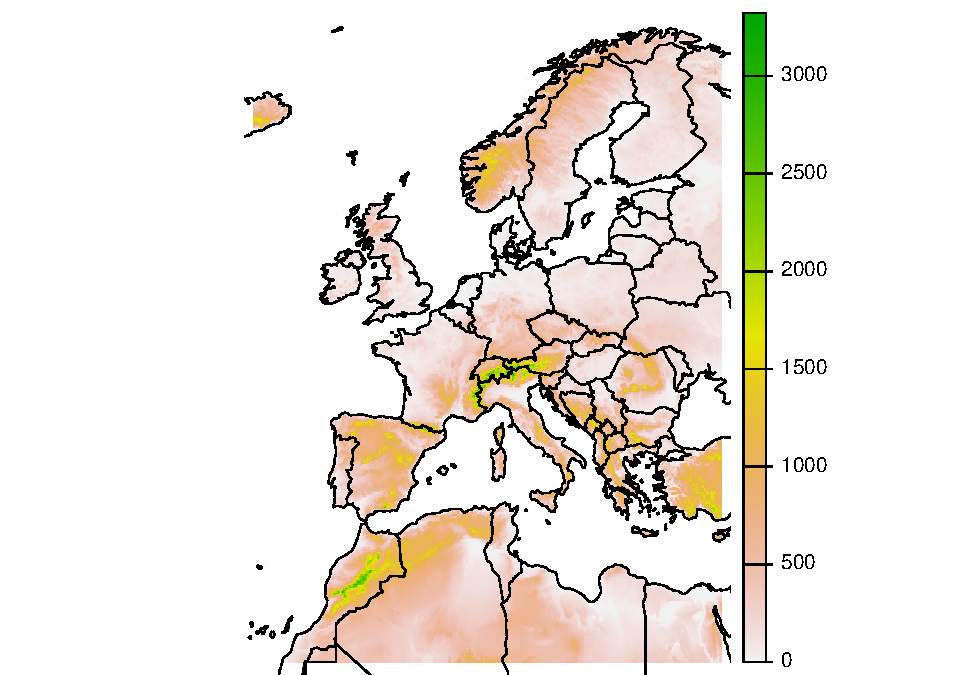
\includegraphics{newsoilsupp_files/figure-latex/firstPlot-2} }\subfloat[night\label{fig:firstPlot-3}]{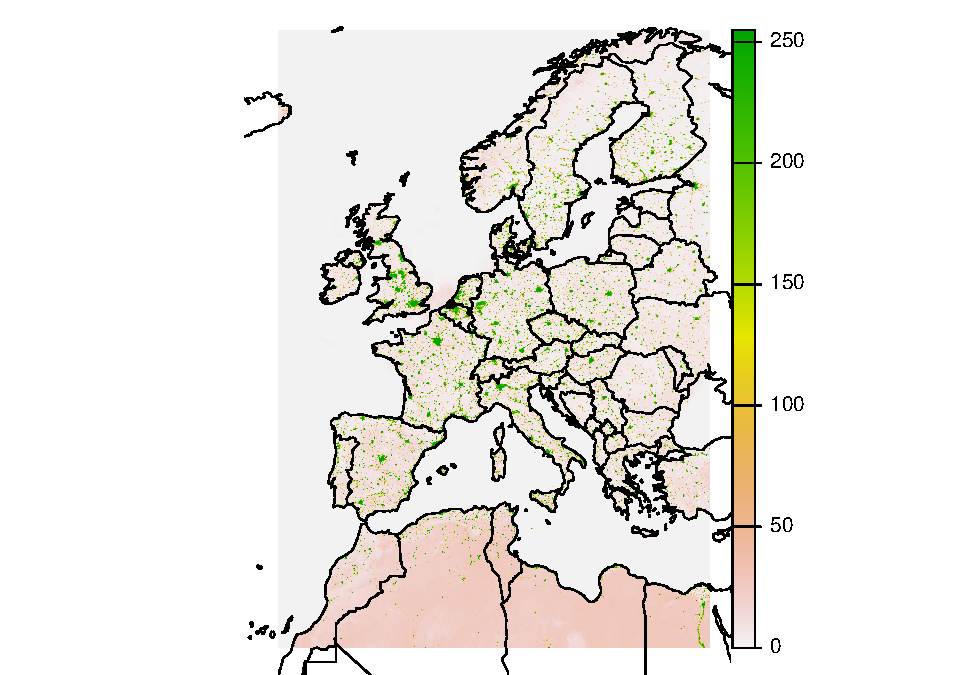
\includegraphics{newsoilsupp_files/figure-latex/firstPlot-3} }\subfloat[evi\label{fig:firstPlot-4}]{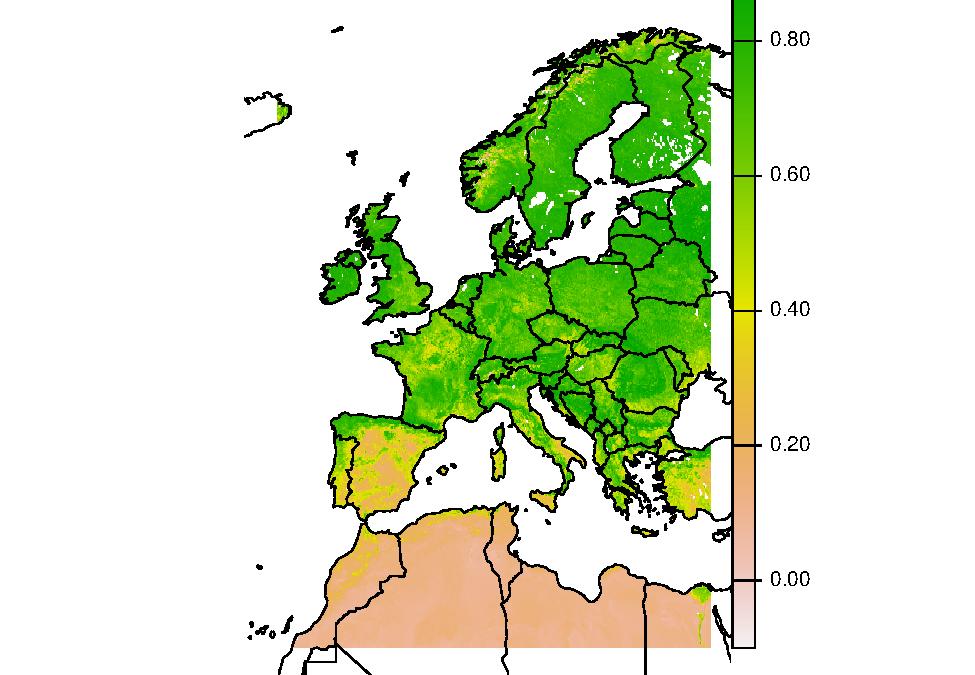
\includegraphics{newsoilsupp_files/figure-latex/firstPlot-4} }\subfloat[land\label{fig:firstPlot-5}]{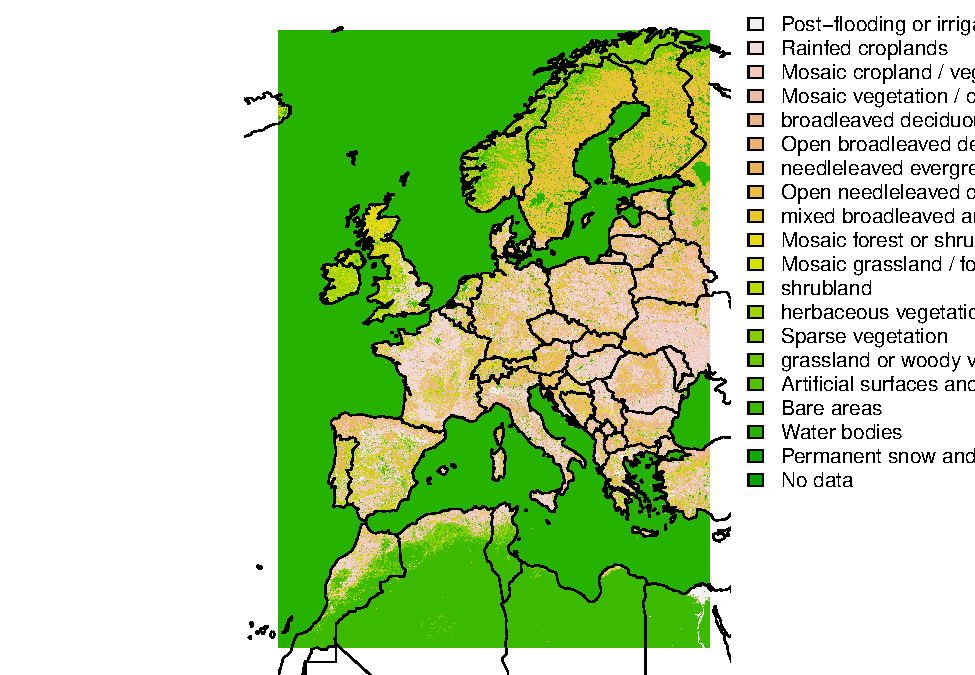
\includegraphics{newsoilsupp_files/figure-latex/firstPlot-5} }\caption{data plot}\label{fig:firstPlot}
\end{figure}

\hypertarget{get-the-mles-on-cpu}{%
\subsection{Get the MLEs on CPU}\label{get-the-mles-on-cpu}}

\begin{Shaded}
\begin{Highlighting}[]
\NormalTok{hgm}\SpecialCharTok{$}\NormalTok{land }\OtherTok{=} \FunctionTok{extract}\NormalTok{(covList}\SpecialCharTok{$}\NormalTok{land, }\FunctionTok{project}\NormalTok{(hgm, }\FunctionTok{crs}\NormalTok{(covList}\SpecialCharTok{$}\NormalTok{land)))[,}\DecValTok{2}\NormalTok{]}
\NormalTok{hgm}\SpecialCharTok{$}\NormalTok{land }\OtherTok{=} \FunctionTok{relevel}\NormalTok{(hgm}\SpecialCharTok{$}\NormalTok{land, }\StringTok{\textquotesingle{}Rainfed croplands\textquotesingle{}}\NormalTok{)}
\FunctionTok{library}\NormalTok{(}\StringTok{\textquotesingle{}geostatsp\textquotesingle{}}\NormalTok{)}
\NormalTok{hgRes }\OtherTok{=} \FunctionTok{lgm}\NormalTok{(HG }\SpecialCharTok{\textasciitilde{}}\NormalTok{ elevation }\SpecialCharTok{+}\NormalTok{ land }\SpecialCharTok{+}\NormalTok{ night }\SpecialCharTok{+}\NormalTok{ evi, }\AttributeTok{data =}\NormalTok{ hgm,}
            \AttributeTok{grid =} \DecValTok{20}\NormalTok{, }\AttributeTok{covariates =}\NormalTok{ covList, }\AttributeTok{fixBoxcox=}\ConstantTok{FALSE}\NormalTok{, }
            \AttributeTok{fixShape=}\ConstantTok{FALSE}\NormalTok{, }\AttributeTok{fixNugget =} \ConstantTok{FALSE}\NormalTok{,  }
            \AttributeTok{reml=}\ConstantTok{FALSE}\NormalTok{, }\AttributeTok{aniso=}\ConstantTok{TRUE}\NormalTok{)}
\end{Highlighting}
\end{Shaded}

\begin{verbatim}
## Warning in krigeLgm(formula = formula, data = data, grid = grid, covariates =
## covariates, : covariates and grid aren't compatible
\end{verbatim}

\begin{Shaded}
\begin{Highlighting}[]
\NormalTok{dataFromLgmWrap }\OtherTok{=} \FunctionTok{wrap}\NormalTok{(hgRes}\SpecialCharTok{$}\NormalTok{data)}

\NormalTok{hgRes2 }\OtherTok{=} \FunctionTok{lgm}\NormalTok{(HG }\SpecialCharTok{\textasciitilde{}}\NormalTok{ elevation }\SpecialCharTok{+}\NormalTok{ land }\SpecialCharTok{+}\NormalTok{ night }\SpecialCharTok{+}\NormalTok{ evi, }\AttributeTok{data =}\NormalTok{ hgm,}
            \AttributeTok{grid =} \DecValTok{20}\NormalTok{, }\AttributeTok{covariates =}\NormalTok{ covList, }\AttributeTok{shape=}\DecValTok{1}\NormalTok{, }
            \AttributeTok{fixBoxcox=}\ConstantTok{FALSE}\NormalTok{, }\AttributeTok{fixShape=}\ConstantTok{TRUE}\NormalTok{, }\AttributeTok{fixNugget =} \ConstantTok{FALSE}\NormalTok{,  }
            \AttributeTok{reml=}\ConstantTok{FALSE}\NormalTok{, }\AttributeTok{aniso=}\ConstantTok{TRUE}\NormalTok{)}
\end{Highlighting}
\end{Shaded}

\begin{verbatim}
## Warning in krigeLgm(formula = formula, data = data, grid = grid, covariates =
## covariates, : covariates and grid aren't compatible
\end{verbatim}

\begin{Shaded}
\begin{Highlighting}[]
\NormalTok{hgRes3 }\OtherTok{=} \FunctionTok{lgm}\NormalTok{(HG }\SpecialCharTok{\textasciitilde{}}\NormalTok{ elevation }\SpecialCharTok{+}\NormalTok{ land }\SpecialCharTok{+}\NormalTok{ night }\SpecialCharTok{+}\NormalTok{ evi, }\AttributeTok{data =}\NormalTok{ hgm,}
             \AttributeTok{grid =} \DecValTok{20}\NormalTok{, }\AttributeTok{covariates =}\NormalTok{ covList, }\AttributeTok{shape=}\FloatTok{0.8}\NormalTok{, }
             \AttributeTok{fixBoxcox=}\ConstantTok{FALSE}\NormalTok{, }\AttributeTok{fixShape=}\ConstantTok{TRUE}\NormalTok{, }\AttributeTok{fixNugget =} \ConstantTok{FALSE}\NormalTok{,  }
             \AttributeTok{reml=}\ConstantTok{FALSE}\NormalTok{, }\AttributeTok{aniso=}\ConstantTok{TRUE}\NormalTok{)}
\end{Highlighting}
\end{Shaded}

\begin{verbatim}
## Warning in krigeLgm(formula = formula, data = data, grid = grid, covariates =
## covariates, : covariates and grid aren't compatible
\end{verbatim}

\begin{Shaded}
\begin{Highlighting}[]
\NormalTok{hgRes4 }\OtherTok{=} \FunctionTok{lgm}\NormalTok{(HG }\SpecialCharTok{\textasciitilde{}}\NormalTok{ elevation }\SpecialCharTok{+}\NormalTok{ land }\SpecialCharTok{+}\NormalTok{ night }\SpecialCharTok{+}\NormalTok{ evi, }\AttributeTok{data =}\NormalTok{ hgm,}
             \AttributeTok{grid =} \DecValTok{20}\NormalTok{, }\AttributeTok{covariates =}\NormalTok{ covList, }\AttributeTok{shape=}\FloatTok{0.5}\NormalTok{, }
             \AttributeTok{fixBoxcox=}\ConstantTok{FALSE}\NormalTok{, }\AttributeTok{fixShape=}\ConstantTok{TRUE}\NormalTok{, }\AttributeTok{fixNugget =} \ConstantTok{FALSE}\NormalTok{,  }
             \AttributeTok{reml=}\ConstantTok{FALSE}\NormalTok{, }\AttributeTok{aniso=}\ConstantTok{TRUE}\NormalTok{)}
\end{Highlighting}
\end{Shaded}

\begin{verbatim}
## Warning in krigeLgm(formula = formula, data = data, grid = grid, covariates =
## covariates, : covariates and grid aren't compatible
\end{verbatim}

\hypertarget{geostatsps-estmates}{%
\subsection{geostatsp's estmates}\label{geostatsps-estmates}}

\begin{Shaded}
\begin{Highlighting}[]
\NormalTok{hgRes}\SpecialCharTok{$}\NormalTok{summary[,}\FunctionTok{c}\NormalTok{(}\StringTok{\textquotesingle{}estimate\textquotesingle{}}\NormalTok{,}\StringTok{\textquotesingle{}ci0.025\textquotesingle{}}\NormalTok{, }\StringTok{\textquotesingle{}ci0.975\textquotesingle{}}\NormalTok{)]}
\end{Highlighting}
\end{Shaded}

\begin{verbatim}
##                                                                                 estimate
## (Intercept)                                                                -7.182301e+00
## elevation                                                                   3.397573e-04
## landbroadleaved deciduous forest                                            0.000000e+00
## landRainfed croplands                                                       3.147825e-01
## landMosaic cropland / vegetation                                            2.202481e-01
## landOpen needleleaved deciduous or evergreen forest                        -3.700127e-01
## landmixed broadleaved and needleleaved forest                              -1.956695e-01
## landMosaic grassland / forest or shrubland                                  1.654901e-01
## landMosaic vegetation / cropland                                           -9.354922e-02
## landSparse vegetation                                                      -7.019042e-01
## landherbaceous vegetation                                                   2.796480e-01
## landMosaic forest or shrubland / grassland                                  4.725326e-02
## landneedleleaved evergreen forest                                           2.669799e-01
## landshrubland                                                               4.647602e-01
## landgrassland or woody vegetation on regularly flooded or waterlogged soil -5.117302e-01
## landArtificial surfaces and associated areas                               -1.118267e-01
## landWater bodies                                                           -8.485128e-01
## night                                                                       1.770369e-03
## evi                                                                         2.556537e+00
## sdNugget                                                                    8.178370e-01
## sdSpatial                                                                   1.489135e+00
## range/1000                                                                  1.374379e+03
## shape                                                                       1.764062e-01
## anisoRatio                                                                  1.181663e+00
## anisoAngleRadians                                                          -9.056046e-01
## anisoAngleDegrees                                                          -5.188732e+01
## boxcox                                                                     -2.305009e-01
##                                                                                  ci0.025
## (Intercept)                                                                -8.419758e+00
## elevation                                                                  -3.698501e-05
## landbroadleaved deciduous forest                                                      NA
## landRainfed croplands                                                      -4.093047e-02
## landMosaic cropland / vegetation                                           -1.178287e-01
## landOpen needleleaved deciduous or evergreen forest                        -8.598177e-01
## landmixed broadleaved and needleleaved forest                              -6.073267e-01
## landMosaic grassland / forest or shrubland                                 -2.246200e-01
## landMosaic vegetation / cropland                                           -4.872423e-01
## landSparse vegetation                                                      -1.180212e+00
## landherbaceous vegetation                                                  -2.753262e-01
## landMosaic forest or shrubland / grassland                                 -5.093636e-01
## landneedleleaved evergreen forest                                          -2.695206e-01
## landshrubland                                                              -2.112822e-01
## landgrassland or woody vegetation on regularly flooded or waterlogged soil -1.327508e+00
## landArtificial surfaces and associated areas                               -1.973410e+00
## landWater bodies                                                           -3.331836e+00
## night                                                                      -1.485800e-04
## evi                                                                         1.427065e+00
## sdNugget                                                                              NA
## sdSpatial                                                                             NA
## range/1000                                                                            NA
## shape                                                                                 NA
## anisoRatio                                                                            NA
## anisoAngleRadians                                                                     NA
## anisoAngleDegrees                                                                     NA
## boxcox                                                                                NA
##                                                                                  ci0.975
## (Intercept)                                                                -5.9448432136
## elevation                                                                   0.0007164996
## landbroadleaved deciduous forest                                                      NA
## landRainfed croplands                                                       0.6704955499
## landMosaic cropland / vegetation                                            0.5583249062
## landOpen needleleaved deciduous or evergreen forest                         0.1197923205
## landmixed broadleaved and needleleaved forest                               0.2159877222
## landMosaic grassland / forest or shrubland                                  0.5556001174
## landMosaic vegetation / cropland                                            0.3001438847
## landSparse vegetation                                                      -0.2235959111
## landherbaceous vegetation                                                   0.8346222640
## landMosaic forest or shrubland / grassland                                  0.6038701034
## landneedleleaved evergreen forest                                           0.8034803390
## landshrubland                                                               1.1408026123
## landgrassland or woody vegetation on regularly flooded or waterlogged soil  0.3040473941
## landArtificial surfaces and associated areas                                1.7497567284
## landWater bodies                                                            1.6348101131
## night                                                                       0.0036893174
## evi                                                                         3.6860089165
## sdNugget                                                                              NA
## sdSpatial                                                                             NA
## range/1000                                                                            NA
## shape                                                                                 NA
## anisoRatio                                                                            NA
## anisoAngleRadians                                                                     NA
## anisoAngleDegrees                                                                     NA
## boxcox                                                                                NA
\end{verbatim}

\begin{Shaded}
\begin{Highlighting}[]
\NormalTok{hgRes}\SpecialCharTok{$}\NormalTok{optim}\SpecialCharTok{$}\NormalTok{logL}
\end{Highlighting}
\end{Shaded}

\begin{verbatim}
## m2logL.ml   logL.ml 
## -3793.079  1896.539
\end{verbatim}

\hypertarget{configure-the-params}{%
\subsection{Configure the params}\label{configure-the-params}}

\begin{Shaded}
\begin{Highlighting}[]
\FunctionTok{library}\NormalTok{(gpuLik)}
\FunctionTok{set.seed}\NormalTok{(}\DecValTok{66}\NormalTok{)}
\NormalTok{alpha1}\OtherTok{=}\FunctionTok{c}\NormalTok{(}\FloatTok{0.00001}\NormalTok{, }\FloatTok{0.01}\NormalTok{, }\FloatTok{0.1}\NormalTok{, }\FloatTok{0.2}\NormalTok{, }\FloatTok{0.25}\NormalTok{, }\FloatTok{0.3}\NormalTok{, }\FloatTok{0.5}\NormalTok{, }\FloatTok{0.8}\NormalTok{, }\FloatTok{0.9}\NormalTok{, }\FloatTok{0.95}\NormalTok{, }\FloatTok{0.99}\NormalTok{, }\FloatTok{0.999}\NormalTok{)}
\NormalTok{alpha2}\OtherTok{=}\FunctionTok{c}\NormalTok{(}\FloatTok{0.00001}\NormalTok{, }\FloatTok{0.01}\NormalTok{, }\FloatTok{0.1}\NormalTok{, }\FloatTok{0.2}\NormalTok{, }\FloatTok{0.5}\NormalTok{, }\FloatTok{0.8}\NormalTok{, }\FloatTok{0.9}\NormalTok{, }\FloatTok{0.95}\NormalTok{, }\FloatTok{0.99}\NormalTok{, }\FloatTok{0.999}\NormalTok{)}

\NormalTok{model\_list }\OtherTok{\textless{}{-}} \FunctionTok{list}\NormalTok{(hgRes, hgRes2, hgRes3, hgRes4)}
\NormalTok{A }\OtherTok{\textless{}{-}}\NormalTok{ gpuLik}\SpecialCharTok{::}\FunctionTok{configParams}\NormalTok{(model\_list, }
                          \AttributeTok{alpha=}\NormalTok{alpha1,}
                          \AttributeTok{alphasecond =}\NormalTok{ alpha2,}
                          \AttributeTok{data =}\NormalTok{ terra}\SpecialCharTok{::}\FunctionTok{unwrap}\NormalTok{(dataFromLgmWrap))}

\NormalTok{paramsUse }\OtherTok{\textless{}{-}}\NormalTok{ A}\SpecialCharTok{$}\NormalTok{representativeParamaters[,}\DecValTok{1}\SpecialCharTok{:}\DecValTok{5}\NormalTok{]}
\NormalTok{b }\OtherTok{\textless{}{-}}\NormalTok{ A}\SpecialCharTok{$}\NormalTok{boxcox}
\end{Highlighting}
\end{Shaded}

\hypertarget{total-number-of-correlation-parameter-sets}{%
\subsection{total number of correlation parameter
sets}\label{total-number-of-correlation-parameter-sets}}

\begin{Shaded}
\begin{Highlighting}[]
\FunctionTok{nrow}\NormalTok{(paramsUse) }
\end{Highlighting}
\end{Shaded}

\begin{verbatim}
## [1] 12316
\end{verbatim}

\hypertarget{section}{%
\subsection{}\label{section}}

\begin{Shaded}
\begin{Highlighting}[]
\CommentTok{\#1}
\NormalTok{intercept}\OtherTok{\textless{}{-}} \FunctionTok{sort}\NormalTok{(}\FunctionTok{c}\NormalTok{(hgRes}\SpecialCharTok{$}\NormalTok{summary[}\StringTok{\textquotesingle{}(Intercept)\textquotesingle{}}\NormalTok{,}\StringTok{\textquotesingle{}estimate\textquotesingle{}}\NormalTok{],}\FunctionTok{seq}\NormalTok{(}\SpecialCharTok{{-}}\DecValTok{10}\NormalTok{, }\SpecialCharTok{{-}}\DecValTok{4}\NormalTok{, }\AttributeTok{len=}\DecValTok{199}\NormalTok{)))}
\CommentTok{\#2}
\NormalTok{elevation  }\OtherTok{\textless{}{-}} \FunctionTok{sort}\NormalTok{(}\FunctionTok{c}\NormalTok{(hgRes}\SpecialCharTok{$}\NormalTok{summary[}\StringTok{\textquotesingle{}elevation\textquotesingle{}}\NormalTok{,}\StringTok{\textquotesingle{}estimate\textquotesingle{}}\NormalTok{], }\FunctionTok{seq}\NormalTok{(}\SpecialCharTok{{-}}\DecValTok{3}\NormalTok{,  }\DecValTok{8}\NormalTok{, }\AttributeTok{len=}\DecValTok{199}\NormalTok{))}\SpecialCharTok{*}\FloatTok{1e{-}04}\NormalTok{)}
\CommentTok{\#3}
\NormalTok{landMosaic\_cropland }\OtherTok{\textless{}{-}} \FunctionTok{sort}\NormalTok{(}\FunctionTok{c}\NormalTok{(hgRes}\SpecialCharTok{$}\NormalTok{summary[}\StringTok{\textquotesingle{}landMosaic cropland / vegetation\textquotesingle{}}\NormalTok{,}\StringTok{\textquotesingle{}estimate\textquotesingle{}}\NormalTok{],}\FunctionTok{seq}\NormalTok{(}\SpecialCharTok{{-}}\FloatTok{0.5}\NormalTok{,  }\FloatTok{0.5}\NormalTok{, }\AttributeTok{len=}\DecValTok{199}\NormalTok{)))  }
\CommentTok{\#4}
\NormalTok{landMosaic\_vegetation }\OtherTok{\textless{}{-}} \FunctionTok{sort}\NormalTok{(}\FunctionTok{c}\NormalTok{(hgRes}\SpecialCharTok{$}\NormalTok{summary[}\StringTok{\textquotesingle{}landMosaic vegetation / cropland\textquotesingle{}}\NormalTok{,}\StringTok{\textquotesingle{}estimate\textquotesingle{}}\NormalTok{],}\FunctionTok{seq}\NormalTok{(}\SpecialCharTok{{-}}\DecValTok{1}\NormalTok{,  }\FloatTok{0.1}\NormalTok{, }\AttributeTok{len=}\DecValTok{199}\NormalTok{))) }
\CommentTok{\#5}
\NormalTok{landbroadleaved\_deciduous\_forest }\OtherTok{\textless{}{-}} \FunctionTok{sort}\NormalTok{(}\FunctionTok{c}\NormalTok{(hgRes}\SpecialCharTok{$}\NormalTok{summary[}\StringTok{\textquotesingle{}landbroadleaved deciduous forest\textquotesingle{}}\NormalTok{,}\StringTok{\textquotesingle{}estimate\textquotesingle{}}\NormalTok{],}\FunctionTok{seq}\NormalTok{(}\SpecialCharTok{{-}}\FloatTok{0.9}\NormalTok{,  }\FloatTok{0.4}\NormalTok{, }\AttributeTok{len=}\DecValTok{199}\NormalTok{)))}
\CommentTok{\#6}
\NormalTok{landneedleleaved\_evergreen\_forest }\OtherTok{\textless{}{-}} \FunctionTok{sort}\NormalTok{(}\FunctionTok{c}\NormalTok{(hgRes}\SpecialCharTok{$}\NormalTok{summary[}\StringTok{\textquotesingle{}landneedleleaved evergreen forest\textquotesingle{}}\NormalTok{,}\StringTok{\textquotesingle{}estimate\textquotesingle{}}\NormalTok{], }\FunctionTok{seq}\NormalTok{(}\SpecialCharTok{{-}}\FloatTok{0.7}\NormalTok{, }\FloatTok{0.8}\NormalTok{, }\AttributeTok{len=}\DecValTok{199}\NormalTok{))) }
\CommentTok{\#7}
\NormalTok{landOpen\_needleleaved\_deciduous\_or\_evergreen\_forest }\OtherTok{\textless{}{-}} \FunctionTok{sort}\NormalTok{(}\FunctionTok{c}\NormalTok{(hgRes}\SpecialCharTok{$}\NormalTok{summary[}\StringTok{\textquotesingle{}landOpen needleleaved deciduous or evergreen forest\textquotesingle{}}\NormalTok{,}\StringTok{\textquotesingle{}estimate\textquotesingle{}}\NormalTok{],}\FunctionTok{seq}\NormalTok{(}\SpecialCharTok{{-}}\FloatTok{1.5}\NormalTok{,  }\DecValTok{0}\NormalTok{, }\AttributeTok{len=}\DecValTok{199}\NormalTok{)))  }
\CommentTok{\#8}
\NormalTok{landmixed\_broadleaved\_and\_needleleaved\_forest }\OtherTok{\textless{}{-}} \FunctionTok{sort}\NormalTok{(}\FunctionTok{c}\NormalTok{(hgRes}\SpecialCharTok{$}\NormalTok{summary[}\StringTok{\textquotesingle{}landmixed broadleaved and needleleaved forest\textquotesingle{}}\NormalTok{,}\StringTok{\textquotesingle{}estimate\textquotesingle{}}\NormalTok{],}\FunctionTok{seq}\NormalTok{(}\SpecialCharTok{{-}}\FloatTok{10.5e{-}01}\NormalTok{, }\SpecialCharTok{{-}}\FloatTok{0.1e{-}01}\NormalTok{, }\AttributeTok{len=}\DecValTok{199}\NormalTok{))) }
\CommentTok{\#9}
\NormalTok{landMosaic\_forest\_or\_shrubland }\OtherTok{\textless{}{-}} \FunctionTok{sort}\NormalTok{(}\FunctionTok{c}\NormalTok{(hgRes}\SpecialCharTok{$}\NormalTok{summary[}\StringTok{\textquotesingle{}landMosaic forest or shrubland / grassland\textquotesingle{}}\NormalTok{,}\StringTok{\textquotesingle{}estimate\textquotesingle{}}\NormalTok{], }\FunctionTok{seq}\NormalTok{(}\SpecialCharTok{{-}}\FloatTok{0.98}\NormalTok{, }\FloatTok{0.4}\NormalTok{, }\AttributeTok{len=}\DecValTok{199}\NormalTok{))) }
\CommentTok{\#10}
\NormalTok{landMosaic\_grassland }\OtherTok{\textless{}{-}} \FunctionTok{sort}\NormalTok{(}\FunctionTok{c}\NormalTok{(hgRes}\SpecialCharTok{$}\NormalTok{summary[}\StringTok{\textquotesingle{}landMosaic grassland / forest or shrubland\textquotesingle{}}\NormalTok{,}\StringTok{\textquotesingle{}estimate\textquotesingle{}}\NormalTok{],}\FunctionTok{seq}\NormalTok{(}\SpecialCharTok{{-}}\FloatTok{0.7}\NormalTok{,  }\FloatTok{0.5}\NormalTok{, }\AttributeTok{len=}\DecValTok{199}\NormalTok{))) }
\CommentTok{\#11}
\NormalTok{landshrubland }\OtherTok{\textless{}{-}} \FunctionTok{sort}\NormalTok{(}\FunctionTok{c}\NormalTok{(hgRes}\SpecialCharTok{$}\NormalTok{summary[}\StringTok{\textquotesingle{}landshrubland\textquotesingle{}}\NormalTok{,}\StringTok{\textquotesingle{}estimate\textquotesingle{}}\NormalTok{], }\FunctionTok{seq}\NormalTok{(}\SpecialCharTok{{-}}\FloatTok{0.6}\NormalTok{, }\FloatTok{0.95}\NormalTok{, }\AttributeTok{len=}\DecValTok{199}\NormalTok{))) }
\CommentTok{\#12}
\NormalTok{landherbaceous\_vegetation  }\OtherTok{\textless{}{-}} \FunctionTok{sort}\NormalTok{(}\FunctionTok{c}\NormalTok{(hgRes}\SpecialCharTok{$}\NormalTok{summary[}\StringTok{\textquotesingle{}landherbaceous vegetation\textquotesingle{}}\NormalTok{,}\StringTok{\textquotesingle{}estimate\textquotesingle{}}\NormalTok{],}\FunctionTok{seq}\NormalTok{(}\SpecialCharTok{{-}}\FloatTok{0.8}\NormalTok{, }\FloatTok{0.7}\NormalTok{, }\AttributeTok{len=}\DecValTok{199}\NormalTok{)))}
\CommentTok{\#13}
\NormalTok{landSparse\_vegetation }\OtherTok{\textless{}{-}} \FunctionTok{sort}\NormalTok{(}\FunctionTok{c}\NormalTok{(hgRes}\SpecialCharTok{$}\NormalTok{summary[}\StringTok{\textquotesingle{}landSparse vegetation\textquotesingle{}}\NormalTok{,}\StringTok{\textquotesingle{}estimate\textquotesingle{}}\NormalTok{],}\FunctionTok{seq}\NormalTok{(}\SpecialCharTok{{-}}\FloatTok{1.8}\NormalTok{, }\FloatTok{0.1}\NormalTok{, }\AttributeTok{len=}\DecValTok{199}\NormalTok{))) }
\CommentTok{\#14}
\NormalTok{landgrassland\_or\_woody\_vegetation }\OtherTok{\textless{}{-}} \FunctionTok{sort}\NormalTok{(}\FunctionTok{c}\NormalTok{(hgRes}\SpecialCharTok{$}\NormalTok{summary[}\StringTok{\textquotesingle{}landgrassland or woody vegetation on regularly flooded or waterlogged soil\textquotesingle{}}\NormalTok{,}\StringTok{\textquotesingle{}estimate\textquotesingle{}}\NormalTok{], }\FunctionTok{seq}\NormalTok{(}\SpecialCharTok{{-}}\FloatTok{1.9}\NormalTok{, }\FloatTok{0.4}\NormalTok{, }\AttributeTok{len=}\DecValTok{199}\NormalTok{))) }
\CommentTok{\#15}
\NormalTok{landArtificial\_surfaces\_and\_associated\_areas  }\OtherTok{\textless{}{-}} \FunctionTok{sort}\NormalTok{(}\FunctionTok{c}\NormalTok{(hgRes}\SpecialCharTok{$}\NormalTok{summary[}\StringTok{\textquotesingle{}landArtificial surfaces and associated areas\textquotesingle{}}\NormalTok{,}\StringTok{\textquotesingle{}estimate\textquotesingle{}}\NormalTok{], }\FunctionTok{seq}\NormalTok{(}\SpecialCharTok{{-}}\FloatTok{2.6}\NormalTok{, }\FloatTok{1.6}\NormalTok{, }\AttributeTok{len=}\DecValTok{199}\NormalTok{)))}
\CommentTok{\#16}
\NormalTok{landWater\_bodies }\OtherTok{\textless{}{-}} \FunctionTok{sort}\NormalTok{(}\FunctionTok{c}\NormalTok{(hgRes}\SpecialCharTok{$}\NormalTok{summary[}\StringTok{\textquotesingle{}landWater bodies\textquotesingle{}}\NormalTok{,}\StringTok{\textquotesingle{}estimate\textquotesingle{}}\NormalTok{], }\FunctionTok{seq}\NormalTok{(}\SpecialCharTok{{-}}\DecValTok{5}\NormalTok{, }\DecValTok{3}\NormalTok{, }\AttributeTok{len=}\DecValTok{199}\NormalTok{)))  }
\CommentTok{\#17}
\NormalTok{night }\OtherTok{\textless{}{-}} \FunctionTok{sort}\NormalTok{(}\FunctionTok{c}\NormalTok{(hgRes}\SpecialCharTok{$}\NormalTok{summary[}\StringTok{\textquotesingle{}night\textquotesingle{}}\NormalTok{,}\StringTok{\textquotesingle{}estimate\textquotesingle{}}\NormalTok{],}\FunctionTok{seq}\NormalTok{(}\SpecialCharTok{{-}}\FloatTok{0.5}\NormalTok{,  }\DecValTok{5}\NormalTok{, }\AttributeTok{len=}\DecValTok{199}\NormalTok{))}\SpecialCharTok{*}\FloatTok{1e{-}03}\NormalTok{) }
\CommentTok{\#18}
\NormalTok{evi }\OtherTok{\textless{}{-}} \FunctionTok{sort}\NormalTok{(}\FunctionTok{c}\NormalTok{(hgRes}\SpecialCharTok{$}\NormalTok{summary[}\StringTok{\textquotesingle{}evi\textquotesingle{}}\NormalTok{,}\StringTok{\textquotesingle{}estimate\textquotesingle{}}\NormalTok{],}\FunctionTok{seq}\NormalTok{(}\DecValTok{0}\NormalTok{,  }\DecValTok{5}\NormalTok{, }\AttributeTok{len=}\DecValTok{199}\NormalTok{)))   }


\NormalTok{Betas }\OtherTok{\textless{}{-}} \FunctionTok{cbind}\NormalTok{(intercept, elevation, landbroadleaved\_deciduous\_forest, }
\NormalTok{               landMosaic\_cropland, }
\NormalTok{               landOpen\_needleleaved\_deciduous\_or\_evergreen\_forest, }
\NormalTok{               landMosaic\_grassland, landMosaic\_vegetation,}
\NormalTok{               landmixed\_broadleaved\_and\_needleleaved\_forest, landSparse\_vegetation, }
\NormalTok{               landherbaceous\_vegetation, landMosaic\_forest\_or\_shrubland,}
\NormalTok{               landneedleleaved\_evergreen\_forest, landshrubland, }
\NormalTok{               landgrassland\_or\_woody\_vegetation, }
\NormalTok{               landArtificial\_surfaces\_and\_associated\_areas,}
\NormalTok{               landWater\_bodies, night, evi)}
\NormalTok{sdSpatial }\OtherTok{\textless{}{-}} \FunctionTok{sort}\NormalTok{(}\FunctionTok{c}\NormalTok{(}\FunctionTok{seq}\NormalTok{(}\FloatTok{0.7}\NormalTok{, }\FloatTok{2.8}\NormalTok{, }\AttributeTok{len=}\DecValTok{59}\NormalTok{), hgRes}\SpecialCharTok{$}\NormalTok{summary[}\StringTok{\textquotesingle{}sdSpatial\textquotesingle{}}\NormalTok{,}\StringTok{\textquotesingle{}estimate\textquotesingle{}}\NormalTok{]))}
\end{Highlighting}
\end{Shaded}

\hypertarget{get-all-estimates-in-a-short-cut-way-may-take-20-25-minutes}{%
\subsection{Get all estimates in a short-cut way (may take 20-25
minutes)}\label{get-all-estimates-in-a-short-cut-way-may-take-20-25-minutes}}

\begin{Shaded}
\begin{Highlighting}[]
\NormalTok{result3}\OtherTok{\textless{}{-}}\NormalTok{gpuLik}\SpecialCharTok{::}\FunctionTok{likfitLgmGpu}\NormalTok{(}\AttributeTok{model=}\NormalTok{hgRes,}
                              \AttributeTok{params=}\NormalTok{paramsUse, }
                              \AttributeTok{data =}\NormalTok{ terra}\SpecialCharTok{::}\FunctionTok{unwrap}\NormalTok{(dataFromLgmWrap),}
                              \AttributeTok{paramToEstimate=}\FunctionTok{c}\NormalTok{(}\StringTok{\textquotesingle{}range\textquotesingle{}}\NormalTok{,}\StringTok{\textquotesingle{}combinedRange\textquotesingle{}}\NormalTok{,}
                                                \StringTok{\textquotesingle{}sdNugget\textquotesingle{}}\NormalTok{,}
                                                \StringTok{\textquotesingle{}shape\textquotesingle{}}\NormalTok{,}\StringTok{\textquotesingle{}nugget\textquotesingle{}}\NormalTok{, }\StringTok{\textquotesingle{}aniso1\textquotesingle{}}\NormalTok{, }
                                                \StringTok{\textquotesingle{}aniso2\textquotesingle{}}\NormalTok{,}\StringTok{\textquotesingle{}boxcox\textquotesingle{}}\NormalTok{),}
                              \AttributeTok{boxcox =} \FunctionTok{seq}\NormalTok{(b[}\DecValTok{1}\NormalTok{],b[}\DecValTok{9}\NormalTok{],}\AttributeTok{len=}\DecValTok{31}\NormalTok{),}
                              \AttributeTok{Betas =}\NormalTok{ Betas,}
                              \AttributeTok{sdSpatial =}\NormalTok{ sdSpatial,}
                              \AttributeTok{cilevel=}\FloatTok{0.95}\NormalTok{,  }\CommentTok{\# decimal}
                              \AttributeTok{type =} \StringTok{"double"}\NormalTok{,}
                              \AttributeTok{NparamPerIter=}\DecValTok{256}\NormalTok{,}\CommentTok{\#400,}
                              \AttributeTok{Nglobal=}\FunctionTok{c}\NormalTok{(}\DecValTok{64}\NormalTok{,}\DecValTok{64}\NormalTok{),    }
                              \AttributeTok{Nlocal=}\FunctionTok{c}\NormalTok{(}\DecValTok{16}\NormalTok{, }\DecValTok{8}\NormalTok{),}\CommentTok{\#c(16,16),}
                              \AttributeTok{NlocalCache=}\DecValTok{2000}\NormalTok{,}\CommentTok{\#2800,}
                              \AttributeTok{verbose=}\FunctionTok{c}\NormalTok{(}\DecValTok{1}\NormalTok{,}\DecValTok{0}\NormalTok{))}
\end{Highlighting}
\end{Shaded}

\begin{verbatim}
## workgroupSize
## 64 64
## localSize
## 16 8
## 
##  Nparams 12316 NparamsPerIter 256 Niter 49 Ncovariates 18 Ndatasets 32 NlocalCacheD 936
\end{verbatim}

\begin{verbatim}
## did not find lower ci for sdNugget
\end{verbatim}

\begin{verbatim}
## did not find lower ci for nugget
\end{verbatim}

\begin{Shaded}
\begin{Highlighting}[]
\FunctionTok{rownames}\NormalTok{(result3}\SpecialCharTok{$}\NormalTok{summary) }\OtherTok{\textless{}{-}} \FunctionTok{substr}\NormalTok{(}\FunctionTok{rownames}\NormalTok{(result3}\SpecialCharTok{$}\NormalTok{summary), }\DecValTok{1}\NormalTok{, }\DecValTok{25}\NormalTok{) }
\end{Highlighting}
\end{Shaded}

\includegraphics[width=0.49\linewidth]{newsoilsupp_files/figure-latex/allestimates-1}
\includegraphics[width=0.49\linewidth]{newsoilsupp_files/figure-latex/allestimates-2}
\includegraphics[width=0.49\linewidth]{newsoilsupp_files/figure-latex/allestimates-3}
\includegraphics[width=0.49\linewidth]{newsoilsupp_files/figure-latex/allestimates-4}
\includegraphics[width=0.49\linewidth]{newsoilsupp_files/figure-latex/allestimates-5}
\includegraphics[width=0.49\linewidth]{newsoilsupp_files/figure-latex/allestimates-6}
\includegraphics[width=0.49\linewidth]{newsoilsupp_files/figure-latex/allestimates-7}
\includegraphics[width=0.49\linewidth]{newsoilsupp_files/figure-latex/allestimates-8}
\includegraphics[width=0.49\linewidth]{newsoilsupp_files/figure-latex/allestimates-9}
\includegraphics[width=0.49\linewidth]{newsoilsupp_files/figure-latex/allestimates-10}
\includegraphics[width=0.49\linewidth]{newsoilsupp_files/figure-latex/allestimates-11}
\includegraphics[width=0.49\linewidth]{newsoilsupp_files/figure-latex/allestimates-12}
\includegraphics[width=0.49\linewidth]{newsoilsupp_files/figure-latex/allestimates-13}
\includegraphics[width=0.49\linewidth]{newsoilsupp_files/figure-latex/allestimates-14}
\includegraphics[width=0.49\linewidth]{newsoilsupp_files/figure-latex/allestimates-15}
\includegraphics[width=0.49\linewidth]{newsoilsupp_files/figure-latex/allestimates-16}
\includegraphics[width=0.49\linewidth]{newsoilsupp_files/figure-latex/allestimates-17}
\includegraphics[width=0.49\linewidth]{newsoilsupp_files/figure-latex/allestimates-18}
\includegraphics[width=0.49\linewidth]{newsoilsupp_files/figure-latex/allestimates-19}
\includegraphics[width=0.49\linewidth]{newsoilsupp_files/figure-latex/allestimates-20}
\includegraphics[width=0.49\linewidth]{newsoilsupp_files/figure-latex/allestimates-21}
\includegraphics[width=0.49\linewidth]{newsoilsupp_files/figure-latex/allestimates-22}
\includegraphics[width=0.49\linewidth]{newsoilsupp_files/figure-latex/allestimates-23}
\includegraphics[width=0.49\linewidth]{newsoilsupp_files/figure-latex/allestimates-24}
\includegraphics[width=0.49\linewidth]{newsoilsupp_files/figure-latex/allestimates-25}
\includegraphics[width=0.49\linewidth]{newsoilsupp_files/figure-latex/allestimates-26}
\includegraphics[width=0.49\linewidth]{newsoilsupp_files/figure-latex/allestimates-27}

\begin{Shaded}
\begin{Highlighting}[]
\NormalTok{result3}\SpecialCharTok{$}\NormalTok{summary}
\end{Highlighting}
\end{Shaded}

\begin{verbatim}
##                                estimate     lower95ci     upper95ci
## (Intercept)               -7.212121e+00 -9.856346e+00 -4.949217e+00
## elevation                  3.388889e-04 -4.700000e-05  7.450000e-04
## landRainfed croplands      3.146465e-01 -4.737119e-02  4.000000e-01
## landMosaic cropland / veg  2.202481e-01 -1.214862e-01  5.000000e-01
## landOpen needleleaved dec -3.636364e-01 -8.937740e-01  0.000000e+00
## landmixed broadleaved and -1.909091e-01 -6.269624e-01  2.198982e-01
## landMosaic grassland / fo  1.000000e-01 -2.356722e-01  1.000000e-01
## landMosaic vegetation / c -9.404040e-02 -4.988000e-01 -1.000000e-02
## landSparse vegetation     -7.019042e-01 -1.242521e+00 -2.123728e-01
## landherbaceous vegetation  2.796480e-01 -2.821208e-01  7.000000e-01
## landMosaic forest or shru  4.725326e-02 -5.197152e-01  4.000000e-01
## landneedleleaved evergree  2.621212e-01 -2.792106e-01  8.000000e-01
## landshrubland              4.646465e-01 -2.178218e-01  9.500000e-01
## landgrassland or woody ve -5.060606e-01 -1.376544e+00  3.108508e-01
## landArtificial surfaces a -1.118267e-01 -2.019217e+00  1.600000e+00
## landWater bodies          -8.485128e-01 -3.433398e+00  1.657199e+00
## night                      1.777778e-03 -1.700000e-04  3.845000e-03
## evi                        2.575758e+00  1.373725e+00  3.916356e+00
## sdSpatial                  1.489135e+00  1.006572e+00  2.800000e+00
## range                      1.374379e+06  3.931983e+05  6.901446e+07
## combinedRange              1.264327e+06  3.446417e+05  6.437687e+07
## sdNugget                   8.311206e-01  0.000000e+00  1.784101e+00
## shape                      1.764062e-01  7.388702e-02  1.140939e+00
## nugget                     3.016235e-01  0.000000e+00  1.402165e+00
## aniso1                    -1.014845e-01 -7.541779e-01  6.683817e-01
## aniso2                    -4.139615e-01 -1.024663e+00  5.915883e-01
## boxcox                    -2.305009e-01 -2.883087e-01 -1.740460e-01
\end{verbatim}

\begin{Shaded}
\begin{Highlighting}[]
\NormalTok{result3}\SpecialCharTok{$}\NormalTok{reml}
\end{Highlighting}
\end{Shaded}

\begin{verbatim}
## [1] FALSE
\end{verbatim}

\hypertarget{or-you-can-do-it-step-by-step-in-the-following-way-showing-only-the-codes-here}{%
\section{Or, you can do it step by step, in the following way, showing
only the codes
here:}\label{or-you-can-do-it-step-by-step-in-the-following-way-showing-only-the-codes-here}}

\hypertarget{get-the-profile-log-likelihoods-only}{%
\subsection{Get the profile log likelihoods
only}\label{get-the-profile-log-likelihoods-only}}

\begin{Shaded}
\begin{Highlighting}[]
\NormalTok{result1 }\OtherTok{\textless{}{-}}\NormalTok{ gpuLik}\SpecialCharTok{::}\FunctionTok{getProfLogL}\NormalTok{(}\AttributeTok{data=}\FunctionTok{unwrap}\NormalTok{(dataFromLgmWrap),}
           \AttributeTok{formula=}\NormalTok{hgRes}\SpecialCharTok{$}\NormalTok{model}\SpecialCharTok{$}\NormalTok{formula,}
           \AttributeTok{coordinates=}\NormalTok{dataFromLgmWrap}\SpecialCharTok{@}\NormalTok{coordinates,}
           \AttributeTok{params=}\NormalTok{paramsUse, }
           \AttributeTok{boxcox =} \FunctionTok{seq}\NormalTok{(b[}\DecValTok{1}\NormalTok{],b[}\DecValTok{9}\NormalTok{],}\AttributeTok{len=}\DecValTok{31}\NormalTok{),}
           \AttributeTok{type =} \StringTok{"double"}\NormalTok{,}
           \AttributeTok{NparamPerIter=}\DecValTok{256}\NormalTok{,}
           \AttributeTok{gpuElementsOnly =} \ConstantTok{FALSE}\NormalTok{,}
           \AttributeTok{reml=}\ConstantTok{FALSE}\NormalTok{, }
           \AttributeTok{Nglobal=}\FunctionTok{c}\NormalTok{(}\DecValTok{256}\NormalTok{,}\DecValTok{256}\NormalTok{),   }
           \AttributeTok{Nlocal=}\FunctionTok{c}\NormalTok{(}\DecValTok{16}\NormalTok{,}\DecValTok{16}\NormalTok{),}
           \AttributeTok{NlocalCache=}\DecValTok{1600}\NormalTok{,}
           \AttributeTok{verbose=}\FunctionTok{c}\NormalTok{(}\DecValTok{1}\NormalTok{,}\DecValTok{0}\NormalTok{))}

\NormalTok{result1}\SpecialCharTok{$}\NormalTok{Infindex}

\NormalTok{result1}\SpecialCharTok{$}\NormalTok{predictors}

\CommentTok{\# gpuLik and geostatsp have same optimal value}
\FunctionTok{max}\NormalTok{(result1}\SpecialCharTok{$}\NormalTok{LogLik)}

\NormalTok{hgRes}\SpecialCharTok{$}\NormalTok{optim}\SpecialCharTok{$}\NormalTok{logL}
\end{Highlighting}
\end{Shaded}

\hypertarget{estimates-and-plots-for-correlation-params}{%
\subsection{Estimates and plots for correlation
params}\label{estimates-and-plots-for-correlation-params}}

\begin{Shaded}
\begin{Highlighting}[]
\NormalTok{result2}\OtherTok{\textless{}{-}}\NormalTok{gpuLik}\SpecialCharTok{::}\FunctionTok{prof1dCov}\NormalTok{(}\AttributeTok{LogLik =}\NormalTok{ result1}\SpecialCharTok{$}\NormalTok{LogLik,  }\CommentTok{\# cpu matrix}
         \AttributeTok{XVYXVX =}\NormalTok{ result1}\SpecialCharTok{$}\NormalTok{XVYXVX,  }\CommentTok{\# cpu matrix}
         \AttributeTok{ssqResidual =}\NormalTok{ result1}\SpecialCharTok{$}\NormalTok{ssqResidual,  }\CommentTok{\# cpu matrix}
         \AttributeTok{paramToEstimate =} \FunctionTok{c}\NormalTok{(}\StringTok{\textquotesingle{}range\textquotesingle{}}\NormalTok{,}\StringTok{\textquotesingle{}combinedRange\textquotesingle{}}\NormalTok{,}\StringTok{\textquotesingle{}shape\textquotesingle{}}\NormalTok{, }\StringTok{\textquotesingle{}sdNugget\textquotesingle{}}\NormalTok{,}
                             \StringTok{\textquotesingle{}nugget\textquotesingle{}}\NormalTok{,}\StringTok{\textquotesingle{}aniso1\textquotesingle{}}\NormalTok{, }\StringTok{\textquotesingle{}aniso2\textquotesingle{}}\NormalTok{,}\StringTok{\textquotesingle{}boxcox\textquotesingle{}}\NormalTok{),}
         \AttributeTok{cilevel=}\FloatTok{0.95}\NormalTok{,  }\CommentTok{\# decimal}
         \AttributeTok{params =}\NormalTok{ result1}\SpecialCharTok{$}\NormalTok{paramsRenew, }\CommentTok{\# cpu matrix,}
         \AttributeTok{boxcox =}\NormalTok{ result1}\SpecialCharTok{$}\NormalTok{boxcox, }
         \AttributeTok{Ndata =}\NormalTok{ result1}\SpecialCharTok{$}\NormalTok{Ndata,}
         \AttributeTok{Nobs =}\NormalTok{ result1}\SpecialCharTok{$}\NormalTok{Nobs,}
         \AttributeTok{Ncov =}\NormalTok{ result1}\SpecialCharTok{$}\NormalTok{Ncov,}
         \AttributeTok{reml =} \ConstantTok{FALSE}\NormalTok{,}
         \AttributeTok{predictors =}\NormalTok{ result1}\SpecialCharTok{$}\NormalTok{predictors,  }\CommentTok{\# character string}
         \AttributeTok{verbose=}\ConstantTok{FALSE}\NormalTok{)}

\CommentTok{\# table of estimates}
\NormalTok{result2}\SpecialCharTok{$}\NormalTok{summary}
\CommentTok{\# index for the MLE parameter set}
\NormalTok{result2}\SpecialCharTok{$}\NormalTok{mleIndex}
\end{Highlighting}
\end{Shaded}

\hypertarget{geostatsps-estmates-1}{%
\subsection{Geostatsp's estmates}\label{geostatsps-estmates-1}}

\begin{Shaded}
\begin{Highlighting}[]
\FunctionTok{rownames}\NormalTok{(hgRes}\SpecialCharTok{$}\NormalTok{summary) }\OtherTok{\textless{}{-}} \FunctionTok{substr}\NormalTok{(}\FunctionTok{rownames}\NormalTok{(hgRes}\SpecialCharTok{$}\NormalTok{summary), }\DecValTok{1}\NormalTok{, }\DecValTok{25}\NormalTok{) }
\NormalTok{hgRes}\SpecialCharTok{$}\NormalTok{summary[,}\FunctionTok{c}\NormalTok{(}\StringTok{\textquotesingle{}estimate\textquotesingle{}}\NormalTok{,}\StringTok{\textquotesingle{}ci0.025\textquotesingle{}}\NormalTok{, }\StringTok{\textquotesingle{}ci0.975\textquotesingle{}}\NormalTok{)]}
\end{Highlighting}
\end{Shaded}

\begin{verbatim}
##                                estimate       ci0.025       ci0.975
## (Intercept)               -7.182301e+00 -8.419758e+00 -5.9448432136
## elevation                  3.397573e-04 -3.698501e-05  0.0007164996
## landbroadleaved deciduous  0.000000e+00            NA            NA
## landRainfed croplands      3.147825e-01 -4.093047e-02  0.6704955499
## landMosaic cropland / veg  2.202481e-01 -1.178287e-01  0.5583249062
## landOpen needleleaved dec -3.700127e-01 -8.598177e-01  0.1197923205
## landmixed broadleaved and -1.956695e-01 -6.073267e-01  0.2159877222
## landMosaic grassland / fo  1.654901e-01 -2.246200e-01  0.5556001174
## landMosaic vegetation / c -9.354922e-02 -4.872423e-01  0.3001438847
## landSparse vegetation     -7.019042e-01 -1.180212e+00 -0.2235959111
## landherbaceous vegetation  2.796480e-01 -2.753262e-01  0.8346222640
## landMosaic forest or shru  4.725326e-02 -5.093636e-01  0.6038701034
## landneedleleaved evergree  2.669799e-01 -2.695206e-01  0.8034803390
## landshrubland              4.647602e-01 -2.112822e-01  1.1408026123
## landgrassland or woody ve -5.117302e-01 -1.327508e+00  0.3040473941
## landArtificial surfaces a -1.118267e-01 -1.973410e+00  1.7497567284
## landWater bodies          -8.485128e-01 -3.331836e+00  1.6348101131
## night                      1.770369e-03 -1.485800e-04  0.0036893174
## evi                        2.556537e+00  1.427065e+00  3.6860089165
## sdNugget                   8.178370e-01            NA            NA
## sdSpatial                  1.489135e+00            NA            NA
## range/1000                 1.374379e+03            NA            NA
## shape                      1.764062e-01            NA            NA
## anisoRatio                 1.181663e+00            NA            NA
## anisoAngleRadians         -9.056046e-01            NA            NA
## anisoAngleDegrees         -5.188732e+01            NA            NA
## boxcox                    -2.305009e-01            NA            NA
\end{verbatim}

\hypertarget{or-get-estimates-for-betas-first-manually-set-the-configuration}{%
\subsection{Or, get estimates for betas first, manually set the
configuration}\label{or-get-estimates-for-betas-first-manually-set-the-configuration}}

\begin{Shaded}
\begin{Highlighting}[]
\CommentTok{\#1}
\NormalTok{intercept}\OtherTok{\textless{}{-}} \FunctionTok{sort}\NormalTok{(}\FunctionTok{c}\NormalTok{(}\SpecialCharTok{{-}}\FloatTok{6.626632}\NormalTok{,}\FunctionTok{seq}\NormalTok{(}\SpecialCharTok{{-}}\DecValTok{10}\NormalTok{, }\SpecialCharTok{{-}}\DecValTok{4}\NormalTok{, }\AttributeTok{len=}\DecValTok{199}\NormalTok{)))}
\CommentTok{\#2}
\NormalTok{elevation  }\OtherTok{\textless{}{-}} \FunctionTok{sort}\NormalTok{(}\FunctionTok{c}\NormalTok{(}\FloatTok{2.7}\NormalTok{,}\FunctionTok{seq}\NormalTok{(}\SpecialCharTok{{-}}\DecValTok{3}\NormalTok{,  }\DecValTok{8}\NormalTok{, }\AttributeTok{len=}\DecValTok{199}\NormalTok{))}\SpecialCharTok{*}\FloatTok{1e{-}04}\NormalTok{)}
\CommentTok{\#3}
\NormalTok{landbroadleaved\_deciduous\_forest }\OtherTok{\textless{}{-}} \FunctionTok{sort}\NormalTok{(}\FunctionTok{c}\NormalTok{(}\SpecialCharTok{{-}}\FloatTok{2.764583e{-}01}\NormalTok{,}\FunctionTok{seq}\NormalTok{(}\SpecialCharTok{{-}}\FloatTok{0.9}\NormalTok{,  }\FloatTok{0.4}\NormalTok{, }\AttributeTok{len=}\DecValTok{199}\NormalTok{)))}
\CommentTok{\#4}
\NormalTok{landMosaic\_cropland }\OtherTok{\textless{}{-}} \FunctionTok{sort}\NormalTok{(}\FunctionTok{c}\NormalTok{(}\SpecialCharTok{{-}}\FloatTok{8.473104e{-}02}\NormalTok{,}\FunctionTok{seq}\NormalTok{(}\SpecialCharTok{{-}}\FloatTok{0.5}\NormalTok{,  }\FloatTok{0.5}\NormalTok{, }\AttributeTok{len=}\DecValTok{199}\NormalTok{)))  }
\CommentTok{\#5}
\NormalTok{landOpen\_needleleaved\_deciduous\_or\_evergreen\_forest }\OtherTok{\textless{}{-}} \FunctionTok{sort}\NormalTok{(}\FunctionTok{c}\NormalTok{(}\SpecialCharTok{{-}}\FloatTok{6.289483e{-}01}\NormalTok{,}\FunctionTok{seq}\NormalTok{(}\SpecialCharTok{{-}}\FloatTok{1.5}\NormalTok{,  }\SpecialCharTok{{-}}\DecValTok{0}\NormalTok{, }\AttributeTok{len=}\DecValTok{199}\NormalTok{)))  }
\CommentTok{\#6}
\NormalTok{landMosaic\_grassland }\OtherTok{\textless{}{-}} \FunctionTok{sort}\NormalTok{(}\FunctionTok{c}\NormalTok{(}\SpecialCharTok{{-}}\FloatTok{8.093025e{-}02}\NormalTok{,}\FunctionTok{seq}\NormalTok{(}\SpecialCharTok{{-}}\FloatTok{0.7}\NormalTok{,  }\FloatTok{0.5}\NormalTok{, }\AttributeTok{len=}\DecValTok{199}\NormalTok{))) }
\CommentTok{\#7}
\NormalTok{landMosaic\_vegetation }\OtherTok{\textless{}{-}} \FunctionTok{sort}\NormalTok{(}\FunctionTok{c}\NormalTok{(}\SpecialCharTok{{-}}\FloatTok{3.748334e{-}01}\NormalTok{,}\FunctionTok{seq}\NormalTok{(}\SpecialCharTok{{-}}\DecValTok{1}\NormalTok{,  }\FloatTok{0.1}\NormalTok{, }\AttributeTok{len=}\DecValTok{199}\NormalTok{))) }
\CommentTok{\#8}
\NormalTok{landmixed\_broadleaved\_and\_needleleaved\_forest }\OtherTok{\textless{}{-}} \FunctionTok{sort}\NormalTok{(}\FunctionTok{c}\NormalTok{(}\SpecialCharTok{{-}}\FloatTok{5.063632e{-}01}\NormalTok{,}\FunctionTok{seq}\NormalTok{(}\SpecialCharTok{{-}}\FloatTok{10.5e{-}01}\NormalTok{, }\SpecialCharTok{{-}}\FloatTok{0.1e{-}01}\NormalTok{, }\AttributeTok{len=}\DecValTok{199}\NormalTok{))) }
\CommentTok{\#9}
\NormalTok{landSparse\_vegetation   }\OtherTok{\textless{}{-}} \FunctionTok{sort}\NormalTok{(}\FunctionTok{c}\NormalTok{(}\SpecialCharTok{{-}}\FloatTok{1.019370e+00}\NormalTok{,}\FunctionTok{seq}\NormalTok{(}\SpecialCharTok{{-}}\FloatTok{1.8}\NormalTok{, }\FloatTok{0.1}\NormalTok{, }\AttributeTok{len=}\DecValTok{199}\NormalTok{)))    }
\CommentTok{\#10}
\NormalTok{landherbaceous\_vegetation  }\OtherTok{\textless{}{-}} \FunctionTok{sort}\NormalTok{(}\FunctionTok{c}\NormalTok{(}\FloatTok{4.877336e{-}03}\NormalTok{,}\FunctionTok{seq}\NormalTok{(}\SpecialCharTok{{-}}\FloatTok{0.8}\NormalTok{, }\FloatTok{0.7}\NormalTok{, }\AttributeTok{len=}\DecValTok{199}\NormalTok{)))  }
\CommentTok{\#11}
\NormalTok{landMosaic\_forest\_or\_shrubland }\OtherTok{\textless{}{-}} \FunctionTok{sort}\NormalTok{(}\FunctionTok{c}\NormalTok{(}\SpecialCharTok{{-}}\FloatTok{2.842735e{-}01}\NormalTok{, }\FunctionTok{seq}\NormalTok{(}\SpecialCharTok{{-}}\FloatTok{0.98}\NormalTok{, }\FloatTok{0.4}\NormalTok{, }\AttributeTok{len=}\DecValTok{199}\NormalTok{)))  }
\CommentTok{\#12}
\NormalTok{landneedleleaved\_evergreen\_forest }\OtherTok{\textless{}{-}} \FunctionTok{sort}\NormalTok{(}\FunctionTok{c}\NormalTok{(}\SpecialCharTok{{-}}\FloatTok{8.919963e{-}03}\NormalTok{, }\FunctionTok{seq}\NormalTok{(}\SpecialCharTok{{-}}\FloatTok{0.7}\NormalTok{, }\FloatTok{0.8}\NormalTok{, }\AttributeTok{len=}\DecValTok{199}\NormalTok{)))  }
\CommentTok{\#13}
\NormalTok{landshrubland }\OtherTok{\textless{}{-}} \FunctionTok{sort}\NormalTok{(}\FunctionTok{c}\NormalTok{(}\FloatTok{2.023893e{-}01}\NormalTok{, }\FunctionTok{seq}\NormalTok{(}\SpecialCharTok{{-}}\FloatTok{0.6}\NormalTok{, }\FloatTok{0.95}\NormalTok{, }\AttributeTok{len=}\DecValTok{199}\NormalTok{)))  }
\CommentTok{\#14}
\NormalTok{landgrassland\_or\_woody\_vegetation }\OtherTok{\textless{}{-}} \FunctionTok{sort}\NormalTok{(}\FunctionTok{c}\NormalTok{(}\SpecialCharTok{{-}}\FloatTok{6.918658e{-}01}\NormalTok{, }\FunctionTok{seq}\NormalTok{(}\SpecialCharTok{{-}}\FloatTok{1.9}\NormalTok{, }\FloatTok{0.4}\NormalTok{, }\AttributeTok{len=}\DecValTok{199}\NormalTok{)))  }
\CommentTok{\#15}
\NormalTok{landArtificial\_surfaces\_and\_associated\_areas  }\OtherTok{\textless{}{-}} \FunctionTok{sort}\NormalTok{(}\FunctionTok{c}\NormalTok{(}\SpecialCharTok{{-}}\FloatTok{4.358506e{-}01}\NormalTok{, }\FunctionTok{seq}\NormalTok{(}\SpecialCharTok{{-}}\FloatTok{2.6}\NormalTok{, }\FloatTok{1.6}\NormalTok{, }\AttributeTok{len=}\DecValTok{199}\NormalTok{))) }
\CommentTok{\#16}
\NormalTok{landWater\_bodies }\OtherTok{\textless{}{-}} \FunctionTok{sort}\NormalTok{(}\FunctionTok{c}\NormalTok{(}\SpecialCharTok{{-}}\FloatTok{1.165791}\NormalTok{, }\FunctionTok{seq}\NormalTok{(}\SpecialCharTok{{-}}\DecValTok{5}\NormalTok{, }\DecValTok{3}\NormalTok{, }\AttributeTok{len=}\DecValTok{199}\NormalTok{)))   }
\CommentTok{\#17}
\NormalTok{night }\OtherTok{\textless{}{-}} \FunctionTok{sort}\NormalTok{(}\FunctionTok{c}\NormalTok{(}\FloatTok{1.560504}\NormalTok{,}\FunctionTok{seq}\NormalTok{(}\SpecialCharTok{{-}}\FloatTok{0.5}\NormalTok{,  }\DecValTok{5}\NormalTok{, }\AttributeTok{len=}\DecValTok{199}\NormalTok{))}\SpecialCharTok{*}\FloatTok{1e{-}03}\NormalTok{) }
\CommentTok{\#18}
\NormalTok{evi }\OtherTok{\textless{}{-}} \FunctionTok{sort}\NormalTok{(}\FunctionTok{c}\NormalTok{(}\FloatTok{2.066869}\NormalTok{,}\FunctionTok{seq}\NormalTok{(}\DecValTok{0}\NormalTok{,  }\DecValTok{5}\NormalTok{, }\AttributeTok{len=}\DecValTok{199}\NormalTok{)))   }


\NormalTok{Betas }\OtherTok{\textless{}{-}} \FunctionTok{cbind}\NormalTok{(intercept, elevation, landbroadleaved\_deciduous\_forest, }
\NormalTok{               landMosaic\_cropland, }
\NormalTok{               landOpen\_needleleaved\_deciduous\_or\_evergreen\_forest, }
\NormalTok{               landMosaic\_grassland, landMosaic\_vegetation,}
\NormalTok{               landmixed\_broadleaved\_and\_needleleaved\_forest, landSparse\_vegetation, }
\NormalTok{               landherbaceous\_vegetation, landMosaic\_forest\_or\_shrubland,}
\NormalTok{               landneedleleaved\_evergreen\_forest, landshrubland, }
\NormalTok{               landgrassland\_or\_woody\_vegetation, }
\NormalTok{               landArtificial\_surfaces\_and\_associated\_areas,}
\NormalTok{               landWater\_bodies, night, evi)}
\end{Highlighting}
\end{Shaded}

\hypertarget{or-automatically-set-the-configuration}{%
\subsection{Or, automatically set the
configuration}\label{or-automatically-set-the-configuration}}

\begin{Shaded}
\begin{Highlighting}[]
\NormalTok{ConfigBetas}\OtherTok{\textless{}{-}}\NormalTok{gpuLik}\SpecialCharTok{::}\FunctionTok{ParamsFromLgm}\NormalTok{(hgRes}\SpecialCharTok{$}\NormalTok{summary,      }\CommentTok{\#lgm model}
             \AttributeTok{covariates=}\NormalTok{result1}\SpecialCharTok{$}\NormalTok{predictors)}

\NormalTok{Betas }\OtherTok{\textless{}{-}}\NormalTok{ ConfigBetas}\SpecialCharTok{$}\NormalTok{Betas }
\end{Highlighting}
\end{Shaded}

\hypertarget{get-estimates-and-profile-plots-for-betas}{%
\subsection{Get estimates and profile plots for
betas'}\label{get-estimates-and-profile-plots-for-betas}}

\begin{Shaded}
\begin{Highlighting}[]
\NormalTok{output}\OtherTok{\textless{}{-}}\NormalTok{gpuLik}\SpecialCharTok{::}\FunctionTok{Prof1dBetas}\NormalTok{(}\AttributeTok{Betas=}\NormalTok{Betas, }
                            \AttributeTok{cilevel=}\FloatTok{0.95}\NormalTok{,}
                            \AttributeTok{Nobs =}\NormalTok{ result1}\SpecialCharTok{$}\NormalTok{Nobs,}
                            \AttributeTok{Ndata =}\NormalTok{ result1}\SpecialCharTok{$}\NormalTok{Ndata,}
                            \AttributeTok{Nparam =}\NormalTok{ result1}\SpecialCharTok{$}\NormalTok{Nparam,}
                            \AttributeTok{Ncov =}\NormalTok{ result1}\SpecialCharTok{$}\NormalTok{Ncov,}
                            \AttributeTok{detVar =}\NormalTok{ result1}\SpecialCharTok{$}\NormalTok{detVar,}
                            \AttributeTok{detReml =}\NormalTok{ result1}\SpecialCharTok{$}\NormalTok{detReml,}
                            \AttributeTok{ssqY =}\NormalTok{ result1}\SpecialCharTok{$}\NormalTok{ssqY,}
                            \AttributeTok{XVYXVX =}\NormalTok{ result1}\SpecialCharTok{$}\NormalTok{XVYXVX,}
                            \AttributeTok{jacobian =}\NormalTok{ result1}\SpecialCharTok{$}\NormalTok{jacobian,}
                            \AttributeTok{reml=}\ConstantTok{FALSE}\NormalTok{,}
                            \AttributeTok{convexHull =} \ConstantTok{FALSE}\NormalTok{)}

\NormalTok{output}\SpecialCharTok{$}\NormalTok{estimates}
\NormalTok{output}\SpecialCharTok{$}\NormalTok{breaks}
\end{Highlighting}
\end{Shaded}

\hypertarget{set-sigma-manually}{%
\subsection{Set sigma manually}\label{set-sigma-manually}}

\begin{Shaded}
\begin{Highlighting}[]
\CommentTok{\#sdSpatial \textless{}{-} sort(c(1.478384, seq(0.7, 2.8, len=59))) }
\NormalTok{sdSpatial }\OtherTok{\textless{}{-}} \FunctionTok{sort}\NormalTok{(}\FunctionTok{seq}\NormalTok{(}\FloatTok{0.7}\NormalTok{, }\FloatTok{2.8}\NormalTok{, }\AttributeTok{len=}\DecValTok{59}\NormalTok{) hgRes}\SpecialCharTok{$}\NormalTok{summary[}\StringTok{\textquotesingle{}sdSpatial\textquotesingle{}}\NormalTok{,}\StringTok{\textquotesingle{}estimate\textquotesingle{}}\NormalTok{])}\ErrorTok{)}
\end{Highlighting}
\end{Shaded}

\hypertarget{or-configure-it-automatically}{%
\subsection{Or, configure it
automatically}\label{or-configure-it-automatically}}

\begin{Shaded}
\begin{Highlighting}[]
\NormalTok{sdSpatial }\OtherTok{\textless{}{-}}\NormalTok{ ConfigBetas}\SpecialCharTok{$}\NormalTok{sdSpatial}
\end{Highlighting}
\end{Shaded}

\hypertarget{estimates-and-profile-plots-for-sdspatial}{%
\subsection{Estimates and profile plots for
sdSpatial}\label{estimates-and-profile-plots-for-sdspatial}}

\begin{Shaded}
\begin{Highlighting}[]
\NormalTok{sdoutput }\OtherTok{\textless{}{-}}\NormalTok{ gpuLik}\SpecialCharTok{::}\FunctionTok{profVariance}\NormalTok{(sdSpatial, }
                                 \AttributeTok{cilevel=}\FloatTok{0.95}\NormalTok{,}
                                 \AttributeTok{Nobs =}\NormalTok{ result1}\SpecialCharTok{$}\NormalTok{Nobs, }
                                 \AttributeTok{Ndata =}\NormalTok{ result1}\SpecialCharTok{$}\NormalTok{Ndata,}
                                 \AttributeTok{Nparam =}\NormalTok{ result1}\SpecialCharTok{$}\NormalTok{Nparam, }
                                 \AttributeTok{Ncov =}\NormalTok{ result1}\SpecialCharTok{$}\NormalTok{Ncov,}
                                 \AttributeTok{detVar =}\NormalTok{ result1}\SpecialCharTok{$}\NormalTok{detVar, }
                                 \AttributeTok{detReml =}\NormalTok{ result1}\SpecialCharTok{$}\NormalTok{detReml, }
                                 \AttributeTok{ssqResidual =}\NormalTok{ result1}\SpecialCharTok{$}\NormalTok{ssqResidual, }
                                 \AttributeTok{jacobian =}\NormalTok{ result1}\SpecialCharTok{$}\NormalTok{jacobian)}

\NormalTok{sdoutput}\SpecialCharTok{$}\NormalTok{estimates}
\NormalTok{breaks }\OtherTok{\textless{}{-}}\NormalTok{ sdoutput}\SpecialCharTok{$}\NormalTok{breaks}

\NormalTok{temp }\OtherTok{\textless{}{-}} \FunctionTok{qchisq}\NormalTok{(}\FloatTok{0.95}\NormalTok{,  }\AttributeTok{df =} \DecValTok{1}\NormalTok{)}\SpecialCharTok{/}\DecValTok{2}
\NormalTok{LogLik }\OtherTok{\textless{}{-}}\NormalTok{ sdoutput}\SpecialCharTok{$}\NormalTok{LogLik}
\NormalTok{breaks }\OtherTok{\textless{}{-}}\NormalTok{ sdoutput}\SpecialCharTok{$}\NormalTok{breaks}

\FunctionTok{plot}\NormalTok{(sdSpatial,LogLik}\SpecialCharTok{{-}}\NormalTok{breaks}\SpecialCharTok{{-}}\NormalTok{temp, }\AttributeTok{cex=}\FloatTok{0.6}\NormalTok{, }\AttributeTok{ylab=}\StringTok{\textquotesingle{}profileLogL\textquotesingle{}}\NormalTok{)}
\FunctionTok{lines}\NormalTok{(sdSpatial,LogLik}\SpecialCharTok{{-}}\NormalTok{breaks}\SpecialCharTok{{-}}\NormalTok{temp, }\AttributeTok{col=}\StringTok{\textquotesingle{}blue\textquotesingle{}}\NormalTok{)}
\FunctionTok{abline}\NormalTok{(}\AttributeTok{h=}\SpecialCharTok{{-}}\NormalTok{temp, }\AttributeTok{lty =} \DecValTok{2}\NormalTok{)}
\FunctionTok{abline}\NormalTok{(}\AttributeTok{v=}\NormalTok{sdoutput}\SpecialCharTok{$}\NormalTok{estimates[}\FunctionTok{c}\NormalTok{(}\DecValTok{1}\NormalTok{,}\DecValTok{2}\NormalTok{,}\DecValTok{3}\NormalTok{)], }\AttributeTok{lty =} \DecValTok{2}\NormalTok{)}
\FunctionTok{text}\NormalTok{(sdoutput}\SpecialCharTok{$}\NormalTok{estimates[}\DecValTok{1}\NormalTok{], }\SpecialCharTok{{-}}\DecValTok{9}\NormalTok{, }\FunctionTok{round}\NormalTok{(sdoutput}\SpecialCharTok{$}\NormalTok{estimates[}\DecValTok{1}\NormalTok{],}\AttributeTok{digits =} \DecValTok{3}\NormalTok{))}
\FunctionTok{text}\NormalTok{(sdoutput}\SpecialCharTok{$}\NormalTok{estimates[}\DecValTok{2}\NormalTok{], }\SpecialCharTok{{-}}\DecValTok{9}\NormalTok{, }\FunctionTok{round}\NormalTok{(sdoutput}\SpecialCharTok{$}\NormalTok{estimates[}\DecValTok{2}\NormalTok{],}\AttributeTok{digits =} \DecValTok{3}\NormalTok{))}
\FunctionTok{text}\NormalTok{(sdoutput}\SpecialCharTok{$}\NormalTok{estimates[}\DecValTok{3}\NormalTok{], }\SpecialCharTok{{-}}\DecValTok{9}\NormalTok{, }\FunctionTok{round}\NormalTok{(sdoutput}\SpecialCharTok{$}\NormalTok{estimates[}\DecValTok{3}\NormalTok{],}\AttributeTok{digits =} \DecValTok{3}\NormalTok{))}
\end{Highlighting}
\end{Shaded}


\end{document}
